\documentclass[border=5mm]{standalone}
\usepackage{luamplib}
\usepackage{graphicx}
\mplibtextextlabel{enable}
\begin{document}

    \begin{mplibcode}

        input segments.mp ;
        input waypoints.mp ;

        beginfig(0);
        picture A,B;
%        A = TEX("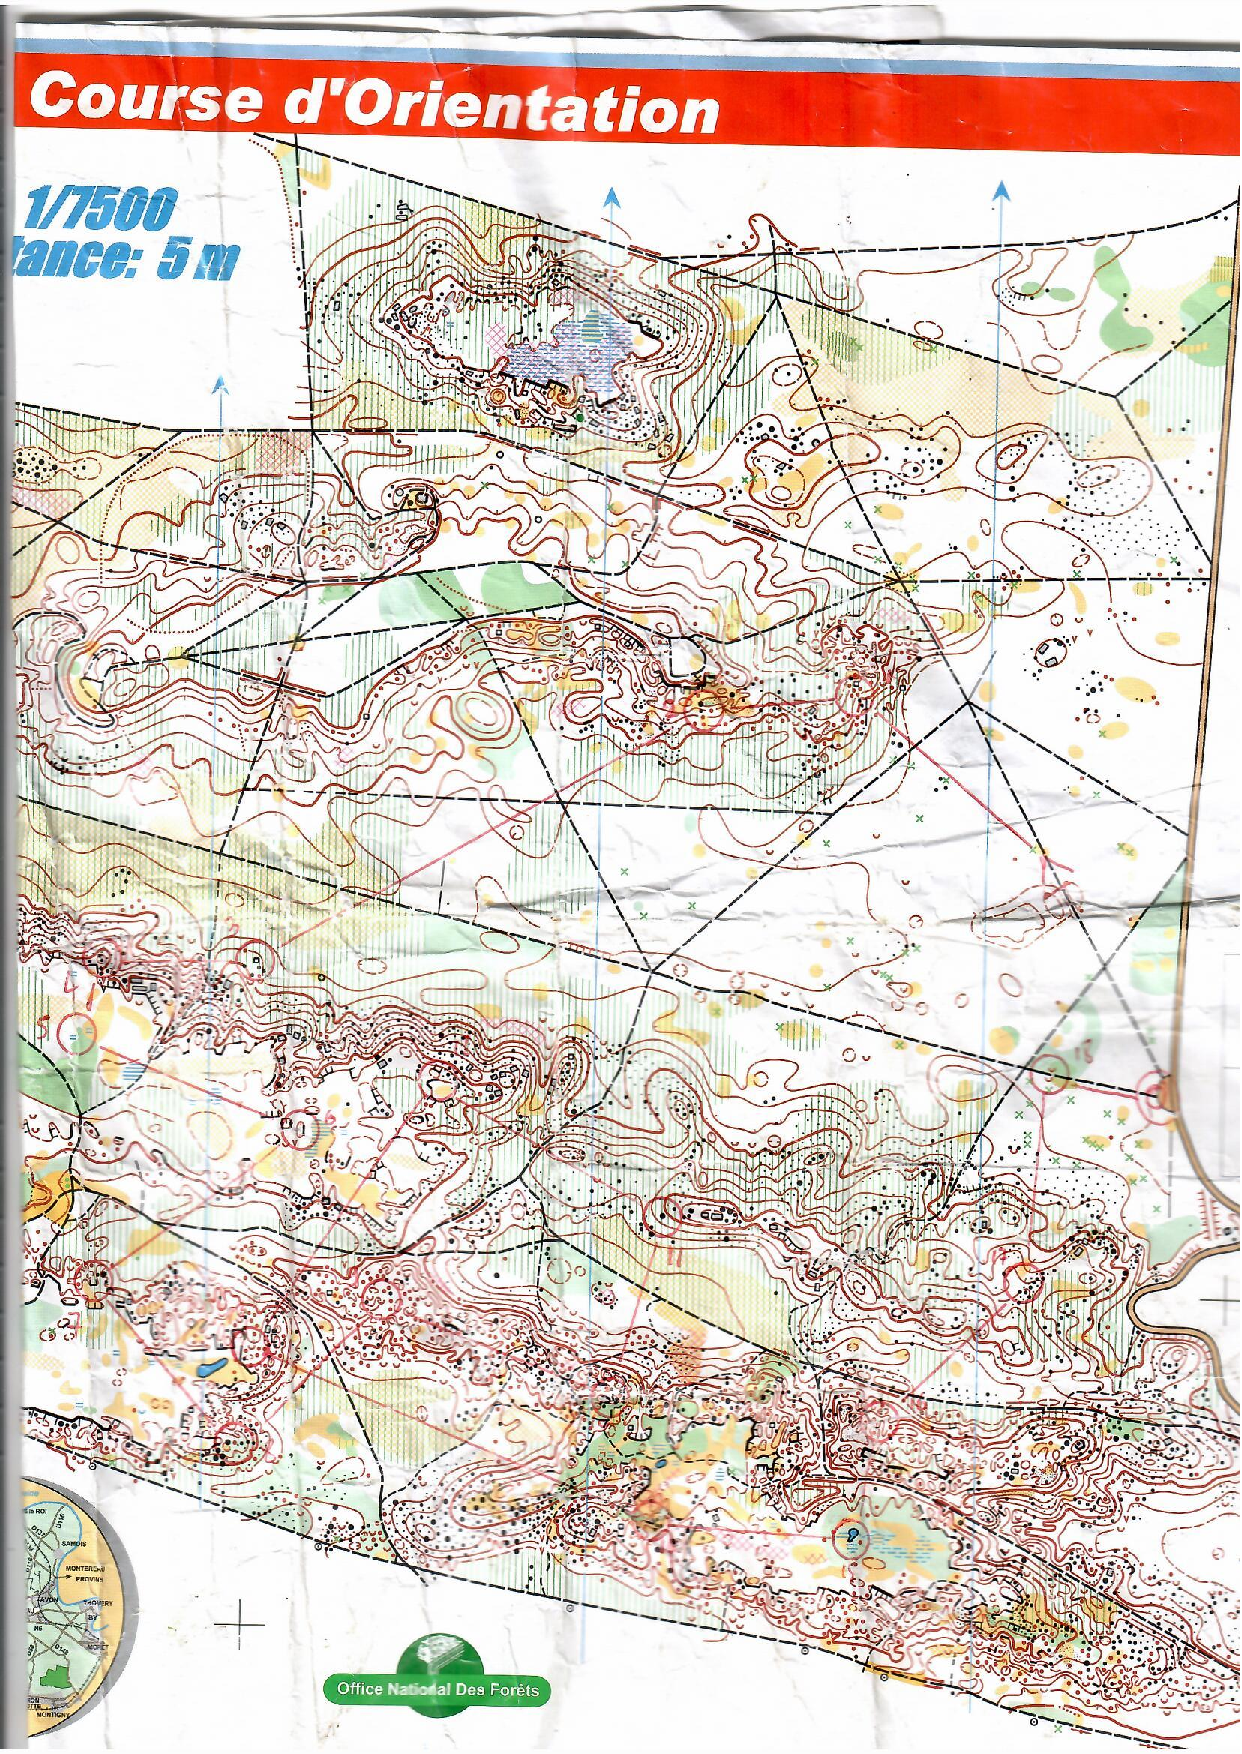
\includegraphics[width=300pt]{le-carrosse-co.pdf}");
        A = TEX("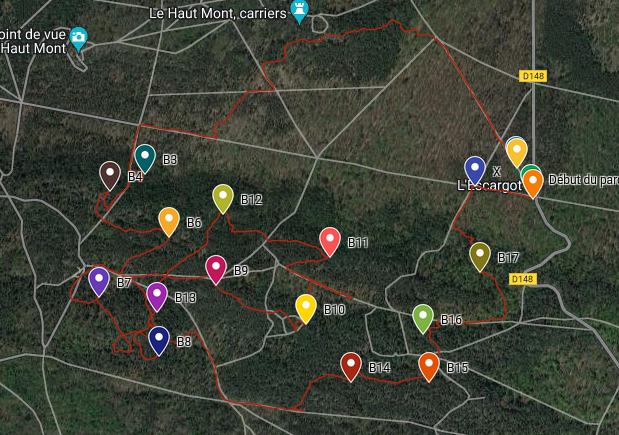
\includegraphics[width=300pt]{le-carrosse-from-google-maps.png}");

        xmin=3 ;
        xmax=10 ;
        ymin = 1.1 ;
        ymax = 10 ;

        %draw A ;
        numeric dx,dy,ratio ;
        dx=0;
        dy=0 ;
        ratio=1 ;
        draw A ;
%    draw B  scaled ratio shifted (dx,dy);

        fill fullcircle scaled 10 withcolor (1,0,0) ;

        path p ;
        transform t ;
        numeric scale,dx,dy;
        scale=1200;
        dx=10.0cm;
        dy=5.3cm ;
        theta=-5 ;
        t := identity scaled scale rotated theta shifted (dx,dy);
        p := get_route(t) ;

        pair pp[] ;
        color pcolor ;
        pcolor = (0,1,0) ;
        draw p withcolor pcolor ;

        pp0 = point 166 of p ;
        draw fullcircle scaled 5 shifted pp0 withcolor pcolor ;
        dotlabel.ulft("0",pp0) withcolor pcolor ;

        pp1 = point 231 of p ;
        draw fullcircle scaled 5 shifted pp1 withcolor pcolor ;
        dotlabel.ulft("1",pp1) withcolor pcolor ;

        pp2 = point 900 of p ;
        draw fullcircle scaled 5 shifted pp2 withcolor pcolor ;
        dotlabel.ulft("2",pp2) withcolor pcolor ;

        pp3 = point 1106 of p ;
        draw fullcircle scaled 5 shifted pp3 withcolor pcolor ;
        dotlabel.ulft("3",pp3) withcolor pcolor ;


        pair qq[] ;
        color qcolor ;
        qcolor=(1,0,0) ;

        qq0 = (134,166) ;
        draw fullcircle scaled 5 shifted qq0 withcolor qcolor ;
        dotlabel.ulft("0",qq0) withcolor qcolor ;

        qq1 = (67,150) ;
        draw fullcircle scaled 5 shifted qq1 withcolor qcolor ;
        dotlabel.ulft("1",qq1) withcolor qcolor ;

        qq2 = (143,13) ;
        draw fullcircle scaled 5 shifted qq2 withcolor qcolor ;
        dotlabel.ulft("2",qq2) withcolor qcolor ;

        qq3 = (228,120) ;
        draw fullcircle scaled 5 shifted qq3 withcolor qcolor ;
        dotlabel.ulft("3",qq3) withcolor qcolor ;


        pickup pencircle scaled 1;
%        draw p withcolor pcolor ;

        transform tt[] ;
%        qq0 = pp0 transformed tt0 ;
        qq1 = pp1 transformed tt0 ;
        qq2 = pp2 transformed tt0 ;
        qq3 = pp3 transformed tt0 ;

        %qq0 = pp0 transformed tt0 ;
%        qq1 = pp1 transformed tt1 ;
%        qq2 = pp2 transformed tt1 ;
%        qq3 = pp3 transformed tt1 ;

        transform chosen_tt ;
        chosen_tt=tt0 ;

        path pp ;
        pp = p transformed chosen_tt ;

        pickup pencircle scaled .1;
        draw pp withcolor (0,1,0) ;

%        draw p transformed tt0 withcolor (0,0,1) ;
        %draw p transformed tt1 withcolor (0,0,1) ;

%        pp = .5[p transformed tt0 ,p  transformed tt1 ] ;
%        draw pp withcolor (1,0,0) ;


        pair wpts[] ;
        get_wpts(wpts)(t) ;
        show "this is wpts" ;
        show wpts ;
        numeric i;
        i=0 ;
        forever:
                exitif unknown wpts[i] ;
                show wpts[i] ;
                pair pwpt ;
%                pwpt = wpts[i] transformed chosen_tt ;
%                draw fullcircle scaled 10 shifted pwpt withcolor (1,0,0) ;
                i:=i+1 ;
        endfor ;


        endfig;

    \end{mplibcode}

\end{document}
